%%%%%%%%%%%%%%%%%%%%%%%%%%%%%%%%%%%%%%%%%
% Beamer Presentation
% LaTeX Template
% Version 1.0 (10/11/12)
%
% This template has been downloaded from:
% http://www.LaTeXTemplates.com
%
% License:
% CC BY-NC-SA 3.0 (http://creativecommons.org/licenses/by-nc-sa/3.0/)
%
%%%%%%%%%%%%%%%%%%%%%%%%%%%%%%%%%%%%%%%%%

%----------------------------------------------------------------------------------------
%	PACKAGES AND THEMES
%----------------------------------------------------------------------------------------

\documentclass{beamer}
\mode<presentation> {

% The Beamer class comes with a number of default slide themes
% which change the colors and layouts of slides. Below this is a list
% of all the themes, uncomment each in turn to see what they look like.

%\usetheme{default}
%\usetheme{AnnArbor}
%\usetheme{Antibes}
%\usetheme{Bergen}
%\usetheme{Berkeley}����JFIF����C
%\usetheme{Berlin}
%\usetheme{Boadilla}
%\usetheme{CambridgeUS}
%\usetheme{Copenhagen}
%\usetheme{Darmstadt}
%\usetheme{Dresden}
%\usetheme{Frankfurt}
%\usetheme{Goettingen}
%\usetheme{Hannover}
%\usetheme{Ilmenau}
%\usetheme{JuanLesPins}
%\usetheme{Luebeck}
%\usetheme{Madrid}
%\usetheme{Malmoe}
%\usetheme{Marburg}
%\usetheme{Montpellier}
\usetheme{PaloAlto}
%\usetheme{Pittsburgh}
%\usetheme{Rochester}
%\usetheme{Singapore}
%\usetheme{Szeged}
%\usetheme{Warsaw}

% As well as themes, the Beamer class has a number of color themes
% for any slide theme. Uncomment each of these in turn to see how it
% changes the colors of your current slide theme.

%\usecolortheme{albatross}
%\usecolortheme{beaver}
%\usecolortheme{beetle}
%\usecolortheme{crane}
%\usecolortheme{dolphin}
%\usecolortheme{dove}
%\usecolortheme{fly}
%\usecolortheme{lily}
%\usecolortheme{orchid}
%\usecolortheme{rose}
%\usecolortheme{seagull}
%\usecolortheme{seahorse}
\usecolortheme{whale}
%\usecolortheme{wolverine}

%\setbeamertemplate{footline} % To remove the footer line in all slides uncomment this line
\setbeamertemplate{footline}[page number] % To replace the footer line in all slides with a simple slide count uncomment this line

%\setbeamertemplate{navigation symbols}{} % To remove the navigation symbols from the bottom of all slides uncomment this line
}

\usepackage{graphicx} % Allows including images
\usepackage{booktabs} % Allows the use of \toprule, \midrule and \bottomrule in tables
\usepackage{amsmath}
\usepackage{subfig}
\usepackage{caption}
\usepackage{mathabx}
\usepackage{wrapfig}
\usepackage{tikz}
\usepackage{animate}
\usetikzlibrary{shapes.geometric, arrows}
%\usepackage{subcaption}
%----------------------------------------------------------------------------------------
%	TITLE PAGE
%----------------------------------------------------------------------------------------
\title[]{Midterm Presentation} % The short title appears at the bottom of every slide, the full title is only on the title page

\author{Group Fleming} % Your name
\institute[University of Twente] % Your institution as it will appear on the bottom of every slide, may be shorthand to save space
{
University of Twente \\ % Your institution for the title page
\medskip
%\textit{john@smith.com} % Your email address
}
\date{\today} % Date, can be changed to a custom date

\begin{document}

\begin{frame}
\titlepage % Print the title page as the first slide
\end{frame}

%----------------------------------------------------------------------------------
\section{Introduction}
\begin{frame}{Folded Dipole with Corner Reflector}
  \begin{columns}[T]
    \begin{column}{.5\textwidth}
     \begin{block}{Requirements:}
\begin{itemize} 
\item	433 MHz transmitting antenna 
\item	Transmitter impedance matching with antenna impedance
\end{itemize}
    \end{block}
    \begin{block}{Objectives:}
\begin{itemize}
\item High gain
\item Design an antenna that works and can be understood
\end{itemize}
\end{block}
    \end{column}
    \begin{column}{.5\textwidth}    
\begin{figure}
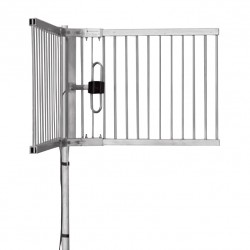
\includegraphics[width=0.7\textwidth]{picture.png}
\cite{figure_of_antenna}
\end{figure}    
    \end{column}
  \end{columns}
\end{frame}

%---------------------------------------------------------------------------
\section{Theory}
\begin{frame}{Hertzian Dipole}
\begin{columns}[T]
    \begin{column}{.7\textwidth}
%\begin{block}
\begin{itemize} 
\item Simplest infinitesimal radiating element
\item Basis for further analysis of more complex antenna
\item Two equal and opposite charge  reservoirs separated by
a distance d 
\item Far field:
\begin{equation*}
B_{\phi} = - \frac{I \: \delta l}{4 \pi j} \left( \frac{e^{-j k r_2}}{r_2} \right) k \sin{(\theta)}
\end{equation*}
\begin{equation*}
E_{\theta} = - \frac{I \: \delta l}{4 \pi j} \left( \frac{e^{-j k r_2}}{r_2} \right) \sqrt{\frac{\mu_0}{\epsilon_0}} \: k \sin{(\theta)}
\end{equation*}
\end{itemize}
%\end{block}
    \end{column}
    \begin{column}{.5\textwidth}    
\begin{figure}
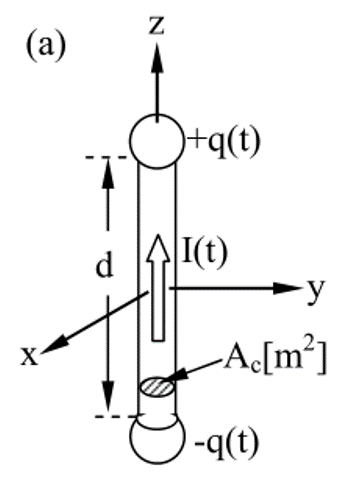
\includegraphics[width=0.5\textwidth]{Hert.png}
\cite{hert}
\end{figure}
    
    \end{column}
  \end{columns}
\end{frame}

%%%%%%%%%%%%%%%%%%%%%%
\begin{frame}{Folded Dipole}
 \begin{block}{Folded Dipole}
 A basic dipole with the two ends folded to make a complete loop
    \end{block}
\begin{columns}[T]
    \begin{column}{.5\textwidth}
\begin{itemize} 
\item	Length of rod are a half wavelength
\item	Direction propagating waves
\end{itemize}
\begin{figure}
\animategraphics[loop,controls,width=0.6\textwidth]{15}{tmp-}{0}{7}
\cite{figure_Waveprop}
\end{figure}
    \end{column}
    \begin{column}{.5\textwidth}    
\begin{figure}
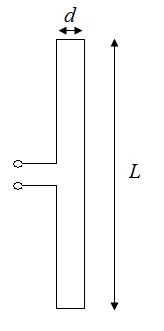
\includegraphics[width=0.4\textwidth]{folded.jpg}
\cite{folded}
\end{figure}
    
    \end{column}
  \end{columns}
\end{frame}


%%%%%%%%%%%%%%%%%
\begin{frame}{Corner Reflector}
\begin{columns}[T]
    \begin{column}{.5\textwidth}
\begin{itemize} 
\item	Increases gain and directivity
\item   Assuming perfectly conducting intersecting planes
\item	Mirrors the dipole, 3 times the signal
\end{itemize}
    \end{column}
    \begin{column}{.5\textwidth}    
\begin{figure}
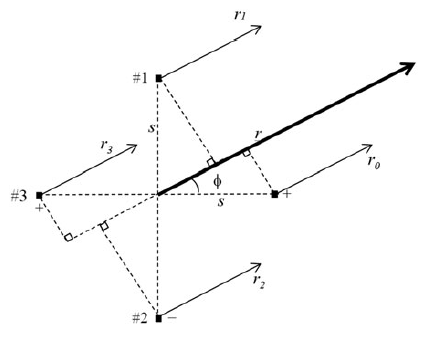
\includegraphics[width=0.9\textwidth]{reflector_image_theory.PNG}
\cite{1_vetharatnam_rashidifar_2015}
%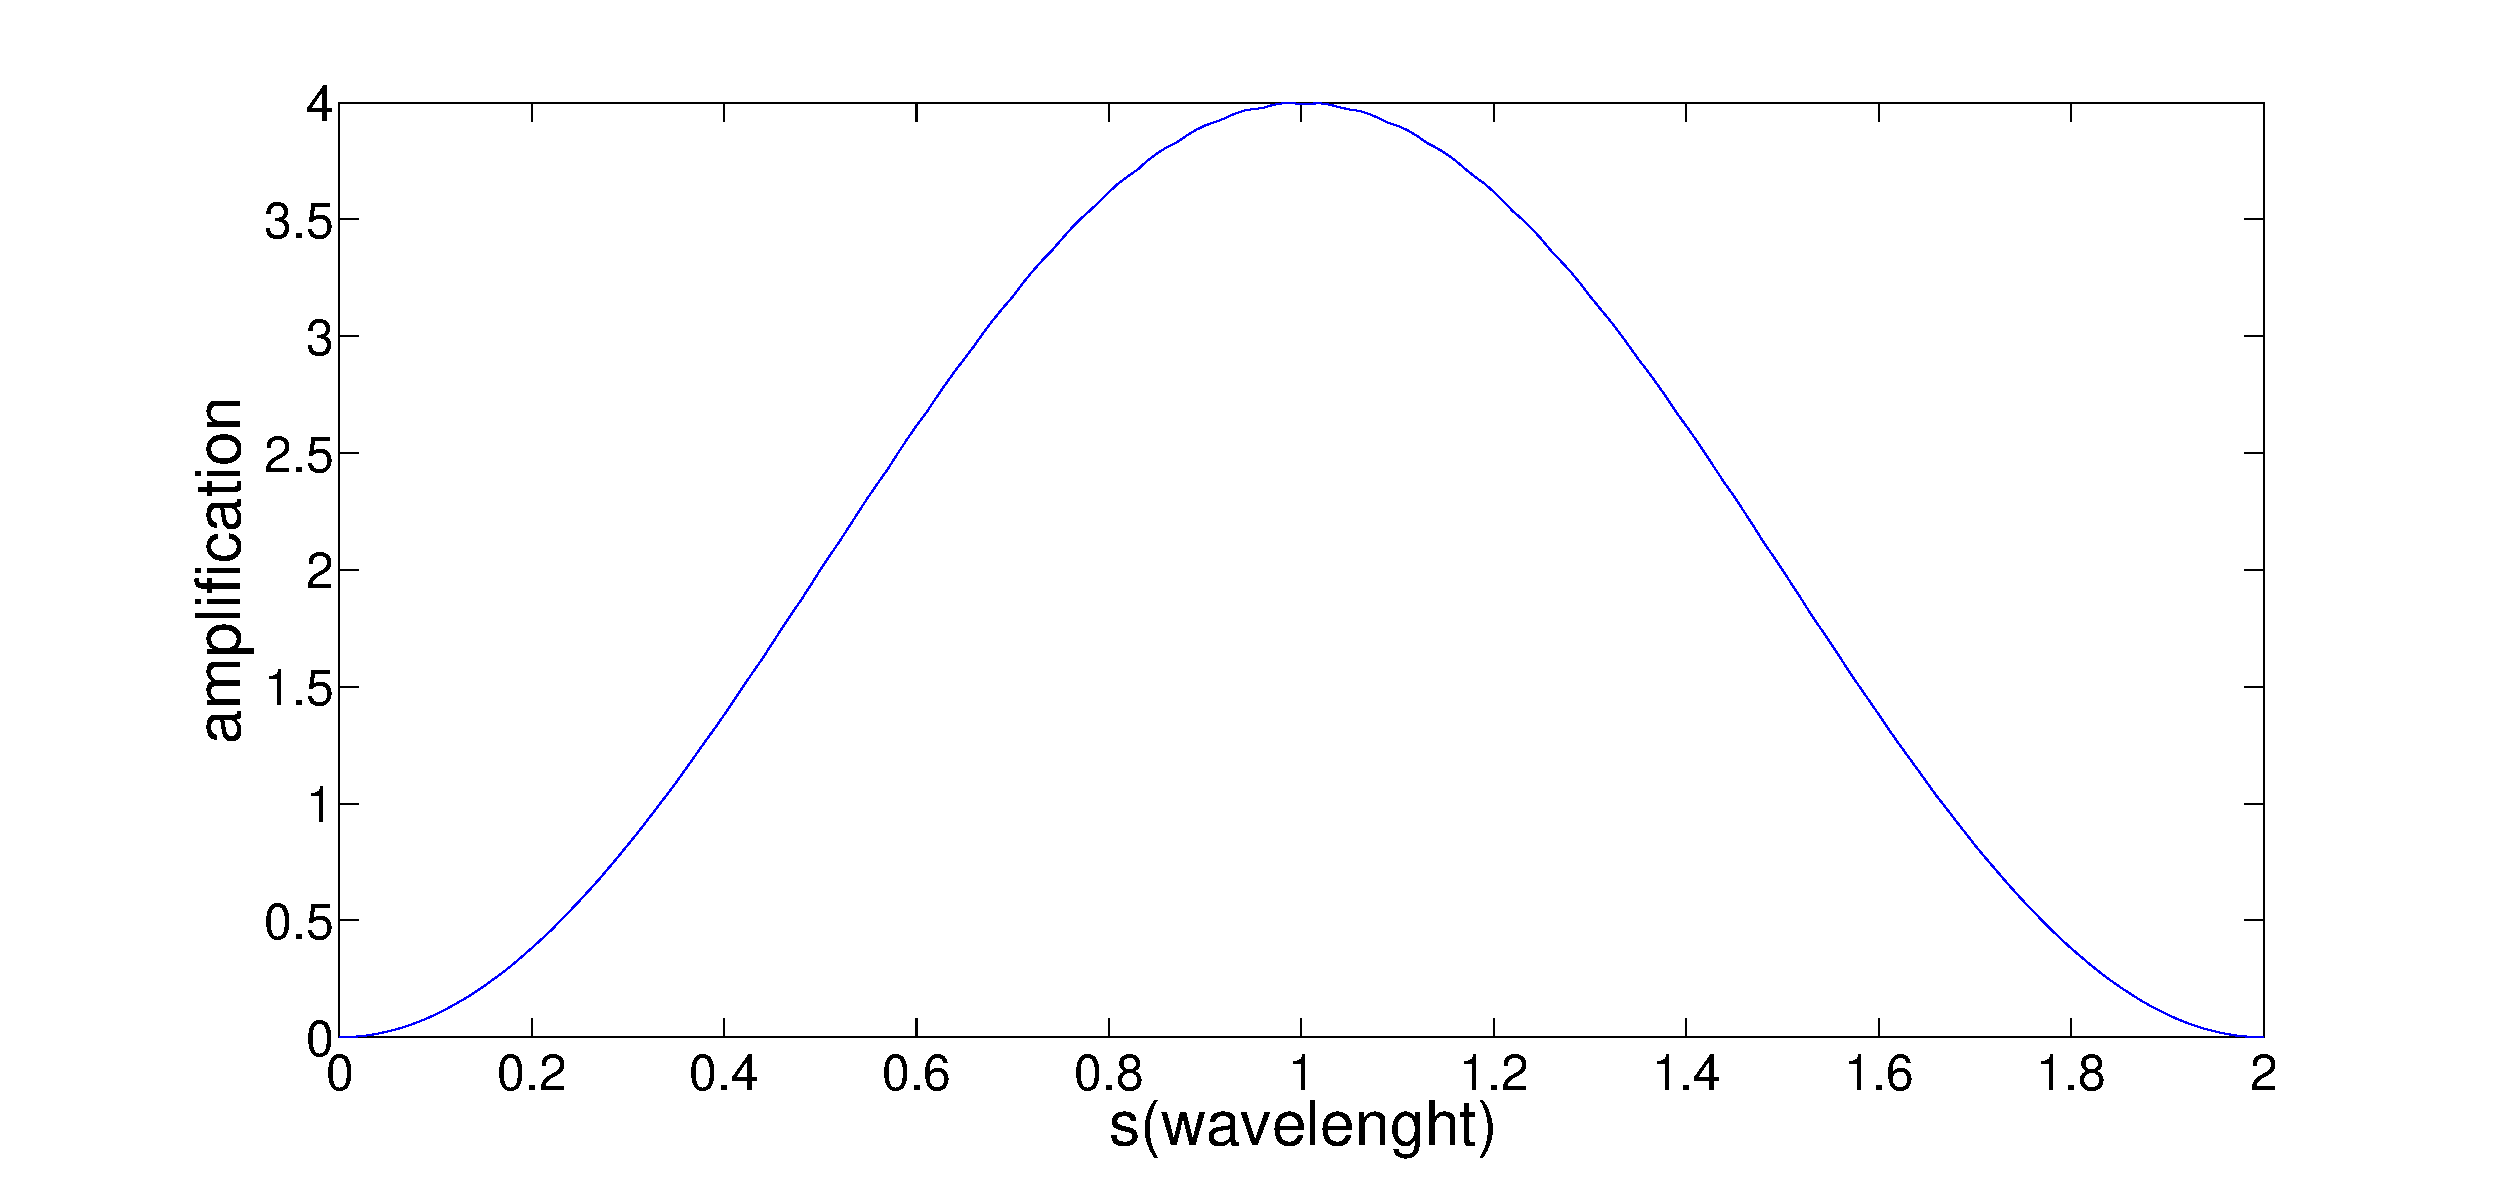
\includegraphics[width=0.8 \textwidth, height=0.3 \textwidth]{Figures/corner_distance.eps}
\end{figure}    
    \end{column}
  \end{columns}
%\item $\vec{E}=f(\theta,\phi) \frac{e^{-jkr}}{r}[2cos(kscos\phi)-2cos(kssin\phi)]$
\end{frame}

%\begin{frame}{Corner Reflector}

%\begin{itemize} 
%\item	Increases gain and directivity
%\item	Mirrors the dipole, 4 times the signal
%\end{itemize}    
%\begin{figure}
%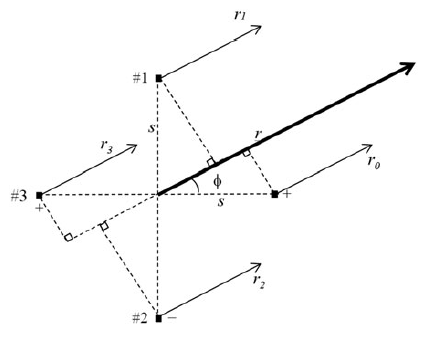
\includegraphics[width=0.8\textwidth]{reflector_image_theory.PNG}
%\cite{1_vetharatnam_rashidifar_2015}
%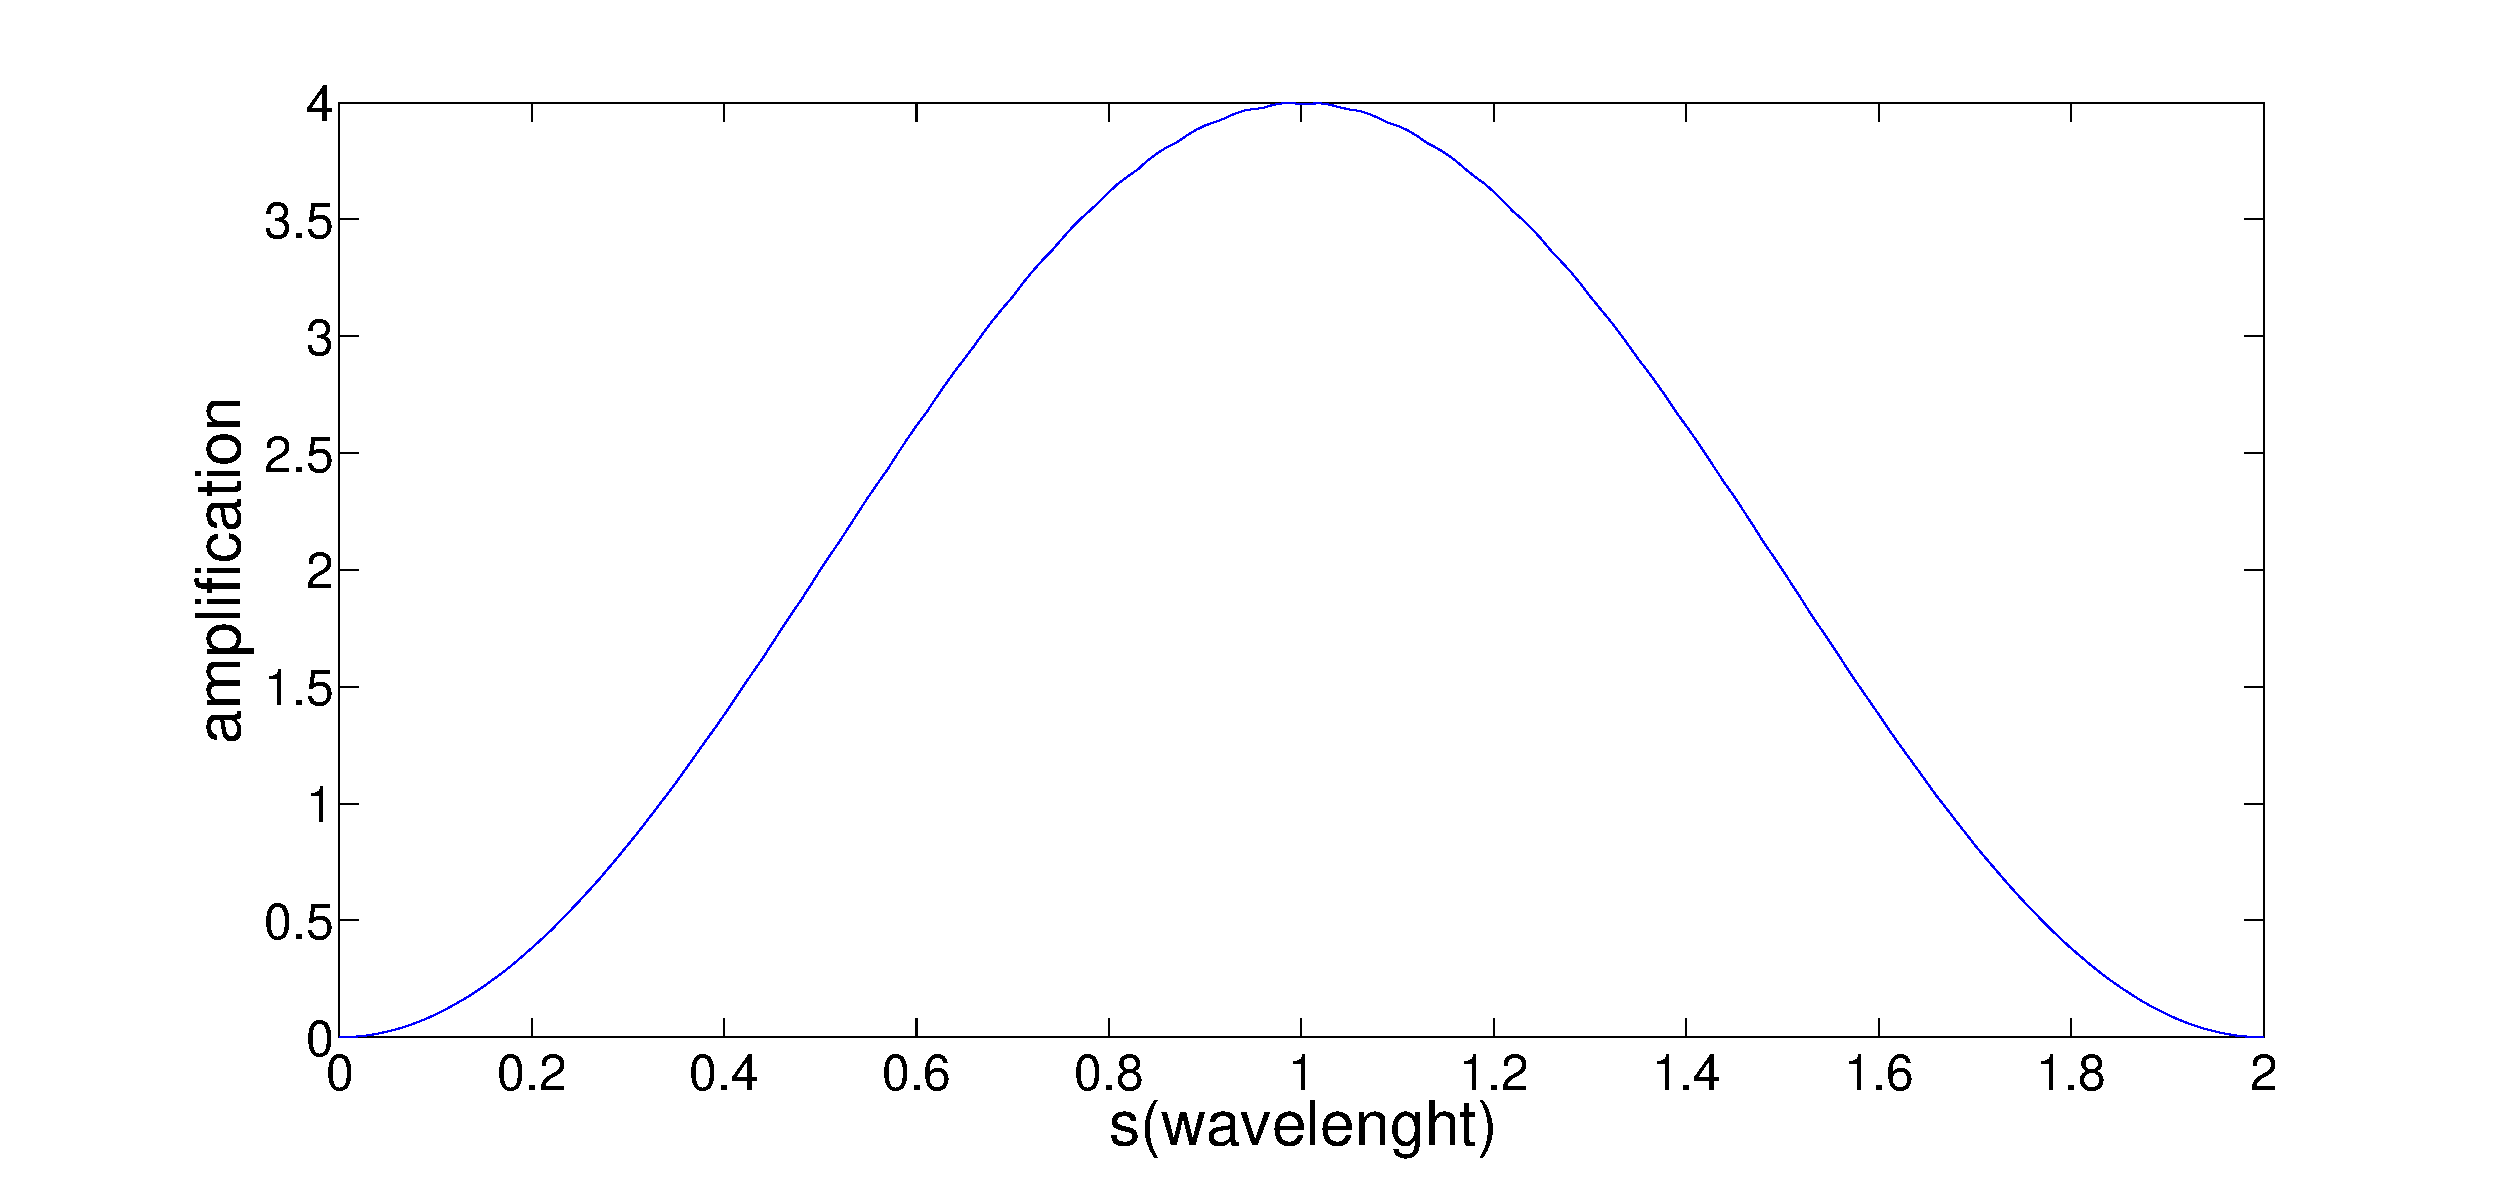
\includegraphics[scale = 0.2]{Figures/corner_distance.eps}
%\end{figure}    
%\end{frame}
%---------------------------------------------------------------------------
%%%%%%%%%%%%%%%%%%%%%%%%%%%%%%%%%%%%%%%%%
\section{Simulations}
\begin{frame}{Simulations vs Calculations}
\begin{columns}[T]
\begin{column}{0.5\textwidth}
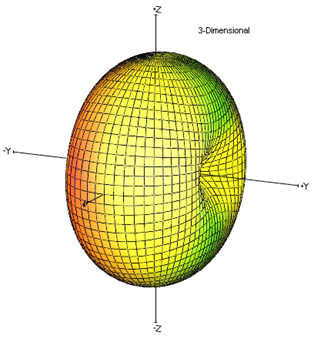
\includegraphics[scale=0.5]{simulation.png}
\end{column}
\begin{column}{0.5\textwidth}
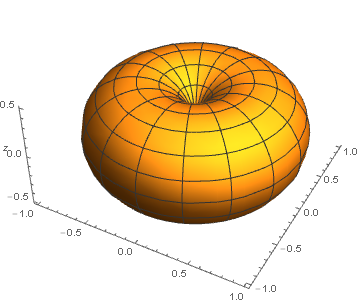
\includegraphics[scale=0.45]{3d.png}
\end{column}
\end{columns}

\end{frame}

%%%%%%%%%%%%%%%%%%%%%%%%%%%%%%%%%%%%%%

\section{Challenges}
\begin{frame}{Issues to Tackle...}
\begin{block}{In theory everything works, but in practice...}
Challenges:
\begin{itemize}
\item Phase
\item Impedance Matching
\item Building
\end{itemize}
\end{block}

\end{frame}
%%%%%%%%%%%
%\begin{frame}{Specifications}
%\begin{itemize}
% \item Operating frequency $433MHz$
%% \item Transmit signal for up to $100m$
% \item Length of Antenna $69 cm$ 4
%\end{itemize}
%\end{frame}
%%%%%%%%%%%
\begin{frame}{Phase}
\begin{itemize}
\item	Desired phase difference of $\pi$
\item We may consider the full-wavelength antenna as composed of two
half-wavelength antennas having identical radiating properties, one excited positively and the other negatively, or $\pi$ out of phase. 
\item 	Phase difference can be regulated by shifting the gap in the dipole 
\end{itemize} 
\end{frame}


%%%%%%%%%%%
\begin{frame}{Impedance Matching}
\begin{block}{}
\begin{itemize}
\item Aim: $Z_{in}=Z_{out}$
\item Minimize the transfer coefficient $\Gamma$
\item ensures that the signal is not reflected back into the transmission line
 \cite{foldeddipolebasics}
\item Maximize the power delivered to the antenna
 \end{itemize}
\end{block}
\begin{itemize}
\item Dependent on the separation between the two dipoles. 
\item Optimum separation smaller than 3 cm. 
\end{itemize}

\end{frame}

%----------------------------------------------------------------------------
\section{Design}
\begin{frame}{Technical Representation}
\begin{figure}
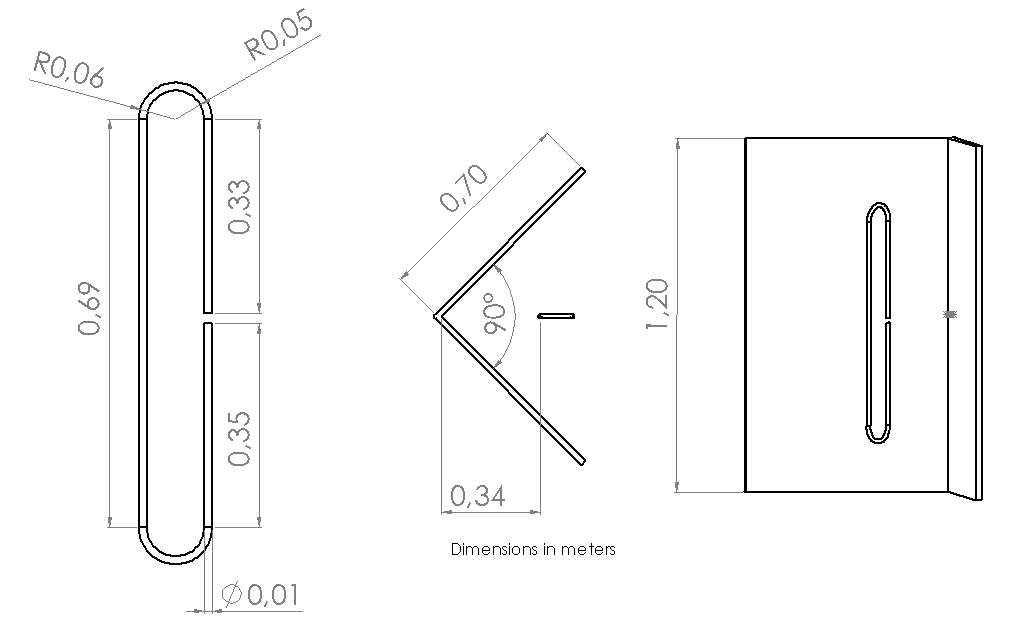
\includegraphics[width=0.9\textwidth]{Folded_dipole_3.PNG}
\end{figure}
\end{frame}

\begin{frame}{Construction}
\begin{itemize}
\item{Building Steps} \\
- Bending a hollow metal pipe to the folded dipole dimensions\\
- Constructing the corner reflector out of wire mesh\\
- Attaching the wires \& balun to the folded dipole\\
\item{Materials}\\
- Copper\\
- Wire mesh\\
- Coax cable\\
- Balun
\item Budget
- 25 euro
\end{itemize}
\end{frame}
%----------------------------------------------------------------------------
\section{Conclusion}
\begin{frame}{Conclusion}
\begin{block}{}
\begin{itemize}
\item	Final calculations
\item	Minor adjustments to size of dipole
\item   Use simulations to verify theory
\item   Take into account that theory is not reality

\end{itemize}
\end{block}


\end{frame}



\begin{frame}{Next Steps}
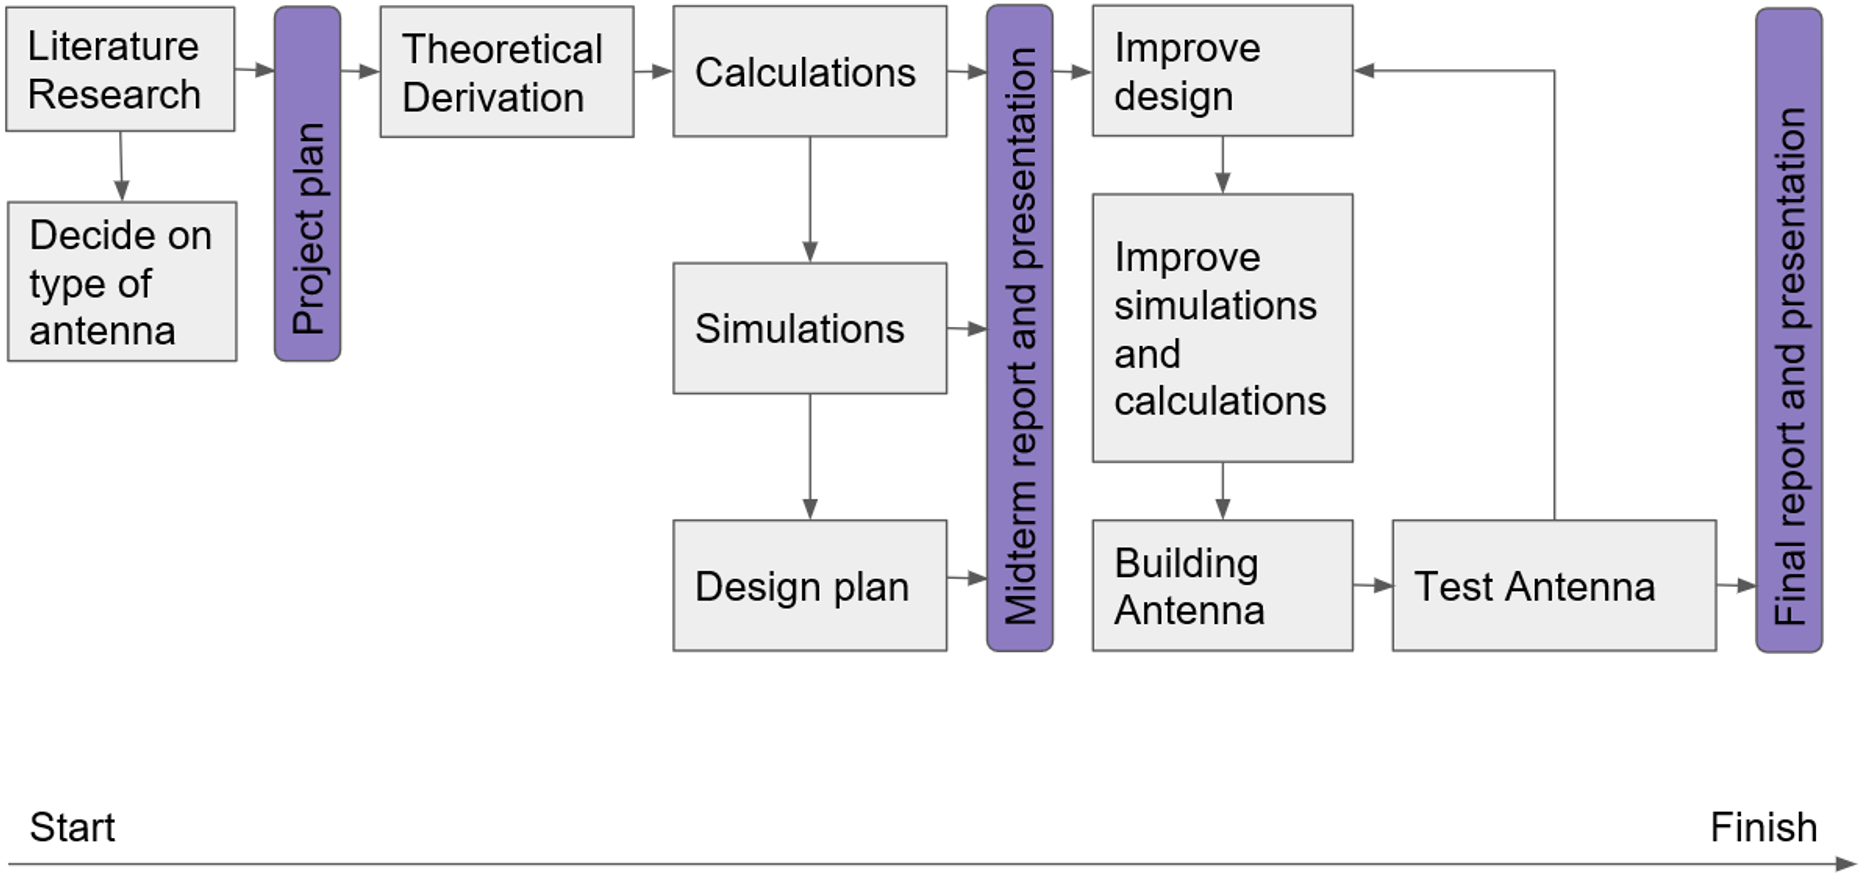
\includegraphics[width=\textwidth]{project_plan_block_diagram.png}
\end{frame}

\begin{frame}[allowframebreaks]{References}
\def\newblock{}
\bibliographystyle{unsrt}
\bibliography{mybib}
\end{frame}
\end{document} 
%---------------------------------------------------------------------------
